%=========================================================================

\chapter{Úvod}
Táto práca je dokumentáciou k samostatnému projektu z predmetu \emph{Aplikovaná kryptografie}. Samostatný projekt sa zaoberá filtrovaním sieťovej prevádzky v systéme GNU/Linux. Cieľom tohto projektu je programovo realizovať aplikáciu, ktorá má na starosť filtrovať zašifrovanú sieťovú prevádzku. Aplikácia má vytvárať štatistiky o type a množstve šifrovaných dát v sieti a ponúknuť možnosť si ich zobraziť v grafickej forme. 

\chapter{Analýza}
V~tejto kapitole je analyzovaná problematika a spôsob riešenia, ktorý je použitý pri tvorbe tejto programovej aplikácie. Dokumentácia predpokladá, že čitateľ pozná koncepty TCP/IP sieťového modelu a Linuxového jadra.

\section{Firewall a filtrovanie}
\emph{Firewall} možno označiť ako ľubovoľné sieťové zariadenie, alebo sieťovú aplikáciu, ktorá slúži k riadeniu sieťovej prevádzky medzi logicky oddelenými sieťami. Podstata firewallu je v predefinovaných pravidlách pre jednotlivé pakety a toky na základe informácii z rôznych vrstiev ISO/OSI modelu. Firewally je možné rozdeliť do nasledujúcich kategórii na základe vývoja počítačových sietí. 

\begin{itemize}
	\itemsep0em 
	\item Paketový filter
	\item Aplikačný filter
	\item Stavový paketový filter
	\item Stavový paketový filter s kontrolou protokolov ľubovoľných vrstiev ISO/OSI modelu
\end{itemize}



\section{Implementácia v Linuxovom jadre}
Moderné Linuxové jadro ponúka granulárnu kontrolu rôznych implementácii firewallu pre filtrovanie sieťových paketov. Práca rozoberá staršiu implementáciu filtrovania pomocou \emph{iptables}, nástupcu vo forme \emph{nftables} a aj firewall následujúcej generácie známy ako \emph{bpfilter}.

\subsection{netfilter}
\emph{netfilter} je možné reprezentovať ako framework Linuxového jadra, slúžiacia pre filtrovanie paketov, preklad sieťových adries alebo preklad sieťových portov. Jeho hlavnú úlohu v jadre plnia hooky, ktoré dovolujú meniť správanie jadra ostatným modulom. Každý paket prechádzajúci kernel prejde cez sadu hookov, ktoré môže zaregistrovať predurčený modul jadra cez callback a následne zareagovať spustením obslužnej procedúry. Netfilter hooking systém obsahuje moduly jadra ako napríklad \texttt{ip\_tables}, \texttt{ip6\_tables}, \texttt{arp\_tables} a \texttt{ebtables}, ktoré možno reprezentovať ako tabuľky pre definíciu pravidiel firewallu. 

\subsection{iptables}
Modul jadra \texttt{ip\_tables} spolu s userspace programom \texttt{iptables} slúži na manipuláciu s tabuľkami \emph{Xtables}, ktoré umožnujú združovať sady pravidiel do reťazcov. Reťazce následne definujú jednotlivé pravidlá pre pakety a sú spracovávané sekvenčne. Pravidlá umožnujú ovyplvňovať priechod sieťovým zásobníkom, kde každý paket musí prejsť aspoň jednou tabuľkou.
\cite{iptables_le}
\begin{figure}[h]
	\centering
	\label{iptables}
	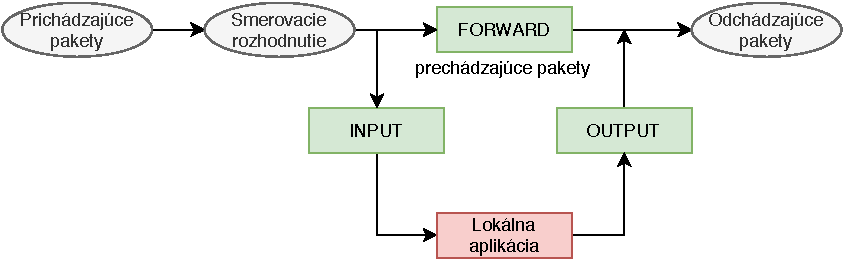
\includegraphics[scale=1.07]{obrazky-figures/iptables.pdf}
	\caption{Základné reťazce \emph{iptables} obsiahnuté v \emph{netfilteri}}
\end{figure}

Hlavným problémom \emph{iptables} a dôvodom zlej reputácie, je primárne vysoká duplicita kódu, nakoľko existuje samostatná tabuľka pre každý sieťový protokol, problémy so škálovaním, rýchlosť spracovávania a mnohé iné

\subsection{nftables}
Náhrada \emph{iptables} vo forme \emph{nftables} je podsystém v Linuxovom jadre, ktorý mení a nahradzuje určité časti samotného \emph{netfilteru}. Základným blokom tohto podsystému je pridanie virtuálneho stroja do Linuxového jadra, ktorý je schopný spúšťať binárny kód určený na prezeranie sieťových paketov a rozhodovanie podľa pravidiel.


\subsection{bpfilter}



\chapter{Záver}
TODO
%=========================================================================
